\section{Numerical Results and Discussion}
To figure out how the number of individuals in each group varies during the GA
process, we conduct one-time experiment and show the number of individuals
in each generation in respect of GA generation. Second, to verify its
performance and stability, the GA is run one hundred times: the best, worst
case, and average results are presented, respectively. Finally, we compare
the results with the work in the other literature.

\begin{figure}[!tb]
	\centering
	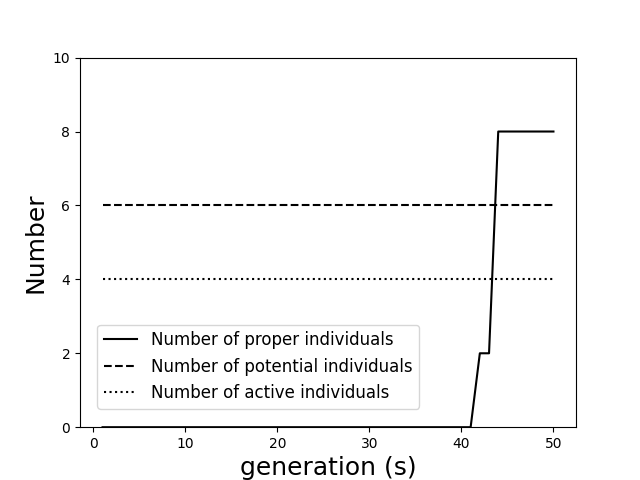
\includegraphics[width=\linewidth]{fig/group_number.png}
	\caption{Number of individuals in each group as a function of generation.}
	\label{fig:group}
\end{figure}

\begin{figure}[!tb]
	\centering
	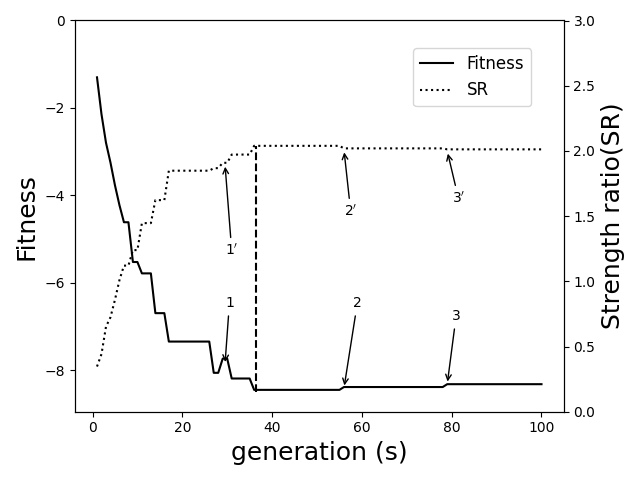
\includegraphics[width=\linewidth]{fig/fitness_strength_ratio.png}
	\caption{The fitness is the negation of the individual's mass. The solid
		curve is the fitness of the best individual in the population in respect
		to the generations; and the dotted line denotes its corresponding strength
		ratio. If no individuals in the population satisfy the constraint, the
		best individual is the one with the biggest strength ratio; if not, the
		best individual is the one with the smallest mass.
}
	\label{fig:sr}
\end{figure}



Fig. \ref{fig:group} shows the number of individuals in each group during the
one-time GA process.  For both active group and potential groups, the number of
individuals is fixed, and equal to its upper bound from the beginning to the
end of the searching process. However, for the proper group, at the initial
stage of GA, no individual fulfills the constraint, so the number of proper
individuals is zero. As seen from Fig. \ref{fig:group}, after forty
generations, proper individuals appear, and its population increases very
quickly up to its upper bound.

There are two approaches that the GA could obtain a better solution: the first
is increasing the length of the chromosome; the second one is adjusting the
internal structure of a chromosome. The GA process can be divided into two
phases by whether there are proper individuals or not. Fig.
\ref{fig:sr} shows the GA process in which the dashed vertical line is the
watershed between the initial phase and the last phase. In the initial phase,
no individual's strength ratio is over the specified threshold, and the main
reason that the fitness gets smaller gradually is the increase of chromosome's
length; At point 1 on the fitness curve, the fitness suddenly goes up, however,
the corresponding strength ratio of point 1, denoted by the point $1^{\prime}$
on the generation-strength ratio curve, also increases. it is because of the
adjustment of a chromosome's layup.  Then GA comes to its second phase. During
this phase, the GA already found proper individuals which could satisfy the
constraint, so the target in this stage is to improve fitness. This means GA
needs to adjust its inner structure, at the point 2 and 3 on the
generation-fitness curve, the fitness curves go up, and the corresponding
strength ratio of these two points slightly go down, but both of them still
satisfy the constraint.


\begin{table*}
\caption{The optimum lay-ups for the loading $N_x=1e^6$ N when changing the value length mutation coefficient, the performance of the GA can be improved when the lenght mutation coefficient is reduced to 1.}
\centering
\begin{adjustbox}{width=1\textwidth}
	\begin{tabular}{cccccccc}
	\toprule
	coefficient		     &	 Material		               	 & case     & Stacking sequence    & Strength ratio  & Mass  &  Cost   & Layer    \\ 
	\midrule																															  
	\multirow{6}{*}{1} &	\multirow{3}{*}{glass-epoxy}   	 & worst     &  $[0_{80}/90_{52}]$ & 2.010           &  8.58  & 132     & 132   \\
						 &								     & best      &  $[0_{75}/90_{43}]$ & 2.000           &  7.67  & 118     & 118  \\
					     &									 & average   &    		           & 2.012           &  7.83  & 123     & 123  \\
						 &	\multirow{3}{*}{graphite-epoxy}	 & worst     &  $[0_{17}/90_{15}]$ & 2.036           & 1.68   & 80      & 32      \\
					     &								     & best      &  $[0_{17}/90_{5}]$  & 2.005           & 1.15   & 55      & 22      \\
					     &								     & average   &                     & 2.018           & 1.47   & 70      & 28      \\
	\multirow{6}{*}{5} &	\multirow{3}{*}{glass-epoxy}   	 & worst     &  $[0_{72}/90_{64}]$ &  2.009          & 8.84   &  136    &  136   \\
						 &								     & best      &  $[0_{72}/90_{53}]$ &  2.003          & 8.12   &  125    &  125   \\
					     &									 & average   &                     &  2.008          & 8.55   &  131    &  131  \\
						 &	\multirow{3}{*}{graphite-epoxy}	 & worst     &  $[0_{18}/90_{24}]$ &  2.006          & 2.20   &  105    &  42  \\
					     &								     & best      &  $[0_{17}/90_{6}]$  &  2.001          & 1.20   &  57     &  23  \\
					     &								     & average   &                    &   2.022          & 1.54   &  73     &  29  \\
	\bottomrule																															  
\end{tabular}
\end{adjustbox}
\label{tab:optimum_layup}
\end{table*}
            
            

Tab. \ref{tab:optimum_layup} shows the searching results after conducting this
experiment one hundred times in two length mutation coefficient cases for
glass-epoxy and graphite-epoxy material, respectively. The best, worst case, and
average experiment results are showed in this table.  For the glass-epoxy
material, if the length mutation coefficient takes one, the best and worst
sequences are $[0_{40}/90_{26}]_s$, $[90_{24}/0_{38}/\bar{90}]_s$; the average mass, cost,
and number of layers are 7.83, 123, 123. If we increase its length mutation
coefficient, suppose it is five, the number of layers for best and worst cases
are 125 and 136;  the average mass, cost, and number of layers are 8.55, 131,
131.  When graphite-epoxy is taken as the experiment material, similar
experiment results are found.  Comparing these two results, we see that a
bigger value of length mutation coefficient can improve this GA's performance.
This is because the mutation coefficient can control both the convergence speed
and search performance, a small mutation coefficient would slow the convergence
speed, however, it would lead to a small-grained exploitation in the local space. 


\begin{table*}[!htb]
\caption{The optimum lay-ups for the loading $N_x=1e6$ N}
\centering
\begin{adjustbox}{width=1\textwidth}
\begin{tabular}{c|cc|cc}
	\toprule
	Cross Ply $[0_M/90_N]$         & \multicolumn{2}{c}{Previous Research} & \multicolumn{2}{c}{Current Research} \\
	\midrule																								  
	 Material       &  Glass-Epoxy & Graphite-Epoxy  & Glass-Epoxy & Graphite-Epoxy      \\ 
	      M         &  68          &    17           &  78		    &  18             \\
	      N         &  72          &    18           &  28		    &  8              \\
no. of lamina(n)    &  140         &    35           &  106	    &  26                     \\
         SR         &  2.01        &    2.10         &  2.03	    &  2.16            \\
     weight         &  9.10        &    1.84         &  6.89	    &  102.5           \\
	\bottomrule
\end{tabular}
\end{adjustbox}
\label{tab:comparsion}
\end{table*}

Tab. \ref{tab:comparsion} shows the optimal cross-ply sequences by the
proposed GA and  Choudhury and Mondal's\cite{choudhury2019failure} study. For
the loading case $Nx=1$ MPa m, the optimal layups are a $[0_{68}/90_{72}]$
cross-ply laminate if glass-epoxy is taken; however, in the present study, a
$[90_{24}/0_{38}/\bar{90}]_s$ glass-epoxy cross-ply laminate is found which
significantly reduces both the cost and weight, and it satisfies the
constraint.  Similarly, if graphite-epoxy is taken, compared with the
$[0_{17}/90_{18}]$ cross-ply laminate, an alternative solution is found,
its layup is $[0_{9}/90_{1}/\bar{0}]_s$. For both cases, we can see that the
experiment results show that using the present proposed GA can obtain better
results.
